У даному розділі досліджено плоска динамічна задача теорії пружності для прямокутної області,
за умов ідеального контакту на бічних гранях.

Вихідна задача зведена до одновимірної задачі у просторі трансформант за допомогою інтегрального перетворення Фур'є.
Отримана крайова задача розв'язана точно за допомогою методу матрично диференціального числення,
фундаментальний розв'язок представлений як інтеграл по замкненому контору, який в свою чергу, був знайденний за допомогою теоремі про лишки.
Остаточний вигляд для функцій переміщеннь та напружень отриман шляхом оберненого перетворення Фур'є.

Проведено чисельний аналіз отриманих функцій переміщень та напружень для різних розмірів прямокутної області та різних видів навантаження.

\subsection{Постановка задачі}
\begin{figure}[h]
    \begin{center}
        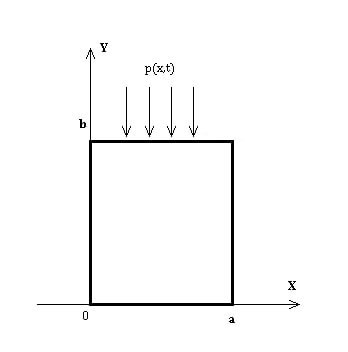
\includegraphics[scale=1]{images/geometry/image_4.jpg}
    \end{center}
    \caption{Геометрія проблеми}\label{geom_dynamic_1}
\end{figure}
Розглядається пружна сама прямокутна область (Рис: \ref{geom_dynamic_1}), яка займає облась,
що описується у декартовій системі координат співвідношенням $0 \le x \le a$, $0 \le y \le b$.

До прямокутної області на грані $y=b$ додане нормальне навантаження
\begin{equation}
    \sigma_y(x, y, t) |_{y=b} = -p(x, t), \quad  \tau_{xy}(x,y,t) |_{y=b} =0
\end{equation}
де $p(x,t)$ відома функція.
На бічних гранях виконується умова ідеального контакту
\begin{equation}
    u(x,y,t) |_{x=0} = 0, \quad \tau_{xy}(x,y,t) |_{x=0} =0
\end{equation}
\begin{equation}
    u(x,y,t) |_{x=a} = 0, \quad \tau_{xy}(x,y,t) |_{x=a} =0
\end{equation}
На нижній грані виконуються наступні умови
\begin{equation}
    v(x,y,t) |_{y=0} = 0, \quad \tau_{xy}(x,y,t) |_{y=0} =0
\end{equation}
Розглядаються наступні рівняння рівноваги Ламе:
\begin{equation}
    \begin{cases}
        \frac{\partial^2 u(x,y,t)}{\partial x^2} + \frac{\partial^2 u(x,y,t)}{\partial y^2} + \mu_0 (\frac{\partial^2 u(x,y,t)}{\partial x^2} + \frac{\partial^2 v(x,y,t)}{\partial x\partial y}) = \frac{1}{c_1^2} \frac{\partial^2 u(x,y,t)}{\partial t^2} \\
        \frac{\partial^2 v(x,y,t)}{\partial x^2} + \frac{\partial^2 v(x,y,t)}{\partial y^2} + \mu_0 (\frac{\partial^2 u(x,y,t)}{\partial x \partial y} + \frac{\partial^2 v(x,y,t)}{\partial y^2}) = \frac{1}{c_2^2} \frac{\partial^2 v(x,y,t)}{\partial t^2} \\
    \end{cases}
\end{equation}

Будемо розглядати випадок гармонічних коливань, тому можемо предствавити функції у наступному вигляді:
\begin{equation}
    u(x,y,t) = u(x,y) e^{i \omega t}, \quad v(x,y,t) = v(x,y) e^{i \omega t}, \quad p(x,t) = p(x) e^{i \omega t}
\end{equation}
Таким чином отримаємо наступні рівняння рівноваги:
\begin{equation}\label{lame_dynamic_1}
    \begin{cases}
        \frac{\partial^2 u(x,y)}{\partial x^2} + \frac{\partial^2 u(x,y)}{\partial y^2} + \mu_0 (\frac{\partial^2 u(x,y)}{\partial x^2} + \frac{\partial^2 v(x,y)}{\partial x\partial y}) = -\frac{\omega^2}{c_1^2}  u(x,y) \\
        \frac{\partial^2 v(x,y)}{\partial x^2} + \frac{\partial^2 v(x,y)}{\partial y^2} + \mu_0 (\frac{\partial^2 u(x,y)}{\partial x \partial y} + \frac{\partial^2 v(x,y)}{\partial y^2}) = -\frac{\omega^2}{c_2^2} v(x,y) \\
    \end{cases}
\end{equation}
Та граничні умови:
\begin{equation}\label{bound_dynamic_1}
    \begin{cases}
        \sigma_y(x, y) |_{y=b} = -p(x, t), \quad  \tau_{xy}(x,y) |_{y=b} =0 \\
        u(x,y) |_{x=0}, \quad \tau_{xy}(x,y) |_{x=0} =0 \\
        u(x,y) |_{x=a}, \quad \tau_{xy}(x,y) |_{x=a} =0 \\
        v(x,y) |_{y=0}, \quad \tau_{xy}(x,y) |_{y=0} =0
    \end{cases}
\end{equation}

\subsection{Зведеня задачі до одновимірної у просторі трансформант}
Для того, щоб звести задачу до одновимірної задачі, використаєм інтегральне перетворення Фур'є по змінній $x$ у до рівнянь (\ref{lame_dynamic_1}) наступному вигляді:
\begin{equation}
    \begin{pmatrix}
        u_n(y) \\
        v_n(y)
    \end{pmatrix} = \int_{0}^{a} 
    \begin{pmatrix}
        u(x,y) sin(\alpha_n x) \\
        v(x,y) cos(\alpha_n x)
    \end{pmatrix} dx, \quad \alpha_n = \frac{\pi n}{a}, n=\overline{1, \infty}
\end{equation}

Для цього помножим перше та друге рівняння (\ref{lame_dynamic_1}) на $sin(\alpha_n x)$ та $cos(\alpha_n x)$ відповідно та проінтегруєм по змінній $x$ на інтервалі $0 \le x \le a$.
Покрокове інтегрування рівняння (\ref{lame_dynamic_1}) наведено у (\nameref{ap_A}).
Отримана система рівнянь задачі у просторі трансформант:
\begin{equation}\label{transf_dynamic_1}
    \begin{cases}
        u_n^{''}(y) - \alpha_n \mu_0 v_n^{'}(y) + (-\alpha_n^2 - -\alpha_n^2 \mu_0 + \frac{\omega^2}{c_1^2}) u_n(y) = 0 \\
        (1 + \mu_0) v_n^{''}(y) + \alpha_n \mu_0 u_n^{'}(y) + (- \alpha_n^2 + \frac{\omega^2}{c_2^2}) v_n(y) = 0 \\
    \end{cases}
\end{equation}

Застосовуючи інтегральне перетворення до граничних умов,
отримаємо наступні умови задачі у просторі трансформант
\begin{equation}\label{transf_bound_dynamic_1}
    \begin{cases}
        \left( (2G + \lambda)v_n^{'}(y) + \alpha_n \lambda u_n(y) \right)|_{y=b} = -p_n \\
        \left(u_n^{'}(y) - \alpha_n v_n(y)  \right)|_{y=b} = 0 \\
        v_n(y)|_{y=0} = 0 \\
        \left(u_n^{'}(y) - \alpha_n v_n(y)  \right)|_{y=0} = 0
    \end{cases}
\end{equation}
Де $p_n = \int_{0}^{a} p(x) cos(\alpha_n x) dx$

\subsection{Зведення задачі у просторі трансформант до матрично-векторної форми}
Для того щоб розв'язати задачу у простосторі трансформант, перепишмо її у матрично-векторній формі.
Рівняння рівноваги (\ref{transf_dynamic_1}) запишемо у наступному вигляді:
\begin{align}\label{transf_mat_dynamic_1}
    &L_2\left[ Z_n(y) \right] = A * Z_n^{''}(y) + B * Z_n^{'}(y) + C * Z_n(y) \nonumber \\
    &L_2\left[ Z_n(y) \right] = 0
\end{align}
Де
\begin{equation*}
    A = \begin{pmatrix}
        1 & 0 \\
        0 & 1 + \mu_0
    \end{pmatrix}, \quad
    B = \begin{pmatrix}
        0 & -\alpha_n \mu_0 \\
        \alpha_n \mu_0 & 0
    \end{pmatrix}
\end{equation*}
\begin{equation*}
    C = \begin{pmatrix}
        -\alpha_n^2 -\alpha_n^2 \mu_0 + \frac{\omega^2}{c_1^2} & 0 \\
        0 & -\alpha_n^2 + \frac{\omega^2}{c_2^2}
    \end{pmatrix}, \quad
    Z_n(y) = \begin{pmatrix}
        u_n(y) \\
        v_n(y)
    \end{pmatrix}
\end{equation*}
Граничні умови (\ref{transf_bound_dynamic_1}) запишемо у наступному вигляді:
\begin{align}\label{transf_bound_mat_dynamic_1}
    &U_i\left[ Z_n(y) \right] = E_i * Z_n^{'}(b_i) + F_i * Z_n(b_i) \nonumber \\
    & U_i\left[ Z_n(y) \right] = D_i
\end{align}
Де $i = \overline{0, 1}$, $b_0 = b$, $b_1 = 0$,
\begin{equation*}
    E_0 = \begin{pmatrix}
        1 & 0 \\
        0 & 2G + \lambda
    \end{pmatrix}, \quad
    F_0 = \begin{pmatrix}
        0 & -\alpha_n \\
        \alpha_n \lambda & 0
    \end{pmatrix}, \quad
\end{equation*}
\begin{equation*}
    E_1 = \begin{pmatrix}
        1 & 0 \\
        0 & 0
    \end{pmatrix}, \quad
    F_1 = \begin{pmatrix}
        0 & -\alpha_n \\
        0 & 1
    \end{pmatrix}, \quad
\end{equation*}
\begin{equation*}
    D_0 = \begin{pmatrix}
        0 \\
        -p_n
    \end{pmatrix}, \quad
    D_1 = \begin{pmatrix}
        0 \\
        0
    \end{pmatrix}, \quad
\end{equation*}

Для знаходження розв'язку задачі у просторі трансформант, знайдем фундаментальну матрицю рівняння (\ref{transf_mat_dynamic_1}).
Шукати її будем у наступному вигляді:
\begin{equation}
    Y(y) = \frac{1}{2\pi i} \oint_C e^{sy} M^{-1}(s)ds
\end{equation}
Де $M(s)$ - характерестична матриця рівняння (\ref{transf_mat_dynamic_1}), а $C$ - замкнений контур який містить усі особливі точки. Яку будемо шукати з наступної умовни
\begin{equation}
    L_2\left[ e^{sy}*I \right] = e^{sy} * M(s), \quad I = \begin{pmatrix} 1 & 0 \\ 0 & 1 \end{pmatrix}
\end{equation}
\begin{align*}
    &L_2\left[ e^{sy}*I \right] = e^{sy} \left( s^2A * I + s B*I + C*I \right) = \\
    &=e^{sy} \begin{pmatrix}
        s^2 - \alpha_n^2 - \alpha_n^2\mu_0 + \frac{\omega^2}{c_1^2} & -\alpha_n \mu_0 s \\
        \alpha_n \mu_0 s & s^2 (1 + \mu_0) -\alpha_n^2 + \frac{\omega^2}{c_1^2}
     \end{pmatrix} =>
\end{align*}

\begin{equation}
    M(s) = \begin{pmatrix}
        s^2 - \alpha_n^2 - \alpha_n^2\mu_0 + \frac{\omega^2}{c_1^2} & -\alpha_n \mu_0 s \\
        \alpha_n \mu_0 s & s^2 (1 + \mu_0) -\alpha_n^2 + \frac{\omega^2}{c_2^2}
     \end{pmatrix}
\end{equation}

Знайдемо тепер $M^{-1}(s) = \frac{\widetilde{M(s)}}{det[M(s)]}$.
\begin{equation}
    \widetilde{M(s)} = \begin{pmatrix}
        s^2 (1 + \mu_0) -\alpha_n^2 + \frac{\omega^2}{c_2^2} & \alpha_n \mu_0 s \\
        -\alpha_n \mu_0 s & s^2 - \alpha_n^2 - \alpha_n^2\mu_0 + \frac{\omega^2}{c_1^2}
     \end{pmatrix}
\end{equation}
\begin{align}
    &det[M(s)] = \begin{vmatrix}
        s^2 - \alpha_n^2 - \alpha_n^2\mu_0 + \frac{\omega^2}{c_1^2} & -\alpha_n \mu_0 s \\
        \alpha_n \mu_0 s & s^2 (1 + \mu_0) -\alpha_n^2 + \frac{\omega^2}{c_2^2}
     \end{vmatrix} = \nonumber \\
    &=(s - s_1)(s + s_1)(s - s_2)(s + s_2)
\end{align}
Де $s_1$, $s_2$, $-s_1$, $-s_2$ корені $det[M(s)]=0$, детальне знаходження яких наведено в (\nameref{ap_B}).

Враховучи це, тепер знайдемо значення фундаментальної матрицю за допомогою теореми про лишки:
\begin{align*}
    &\frac{1}{2\pi i} \oint_C e^{sy} M^{-1}(s)ds = \frac{2 \pi i}{2 \pi i (1 + \mu_0)} \sum_{i=1}^{4} Res\left[ e^{sy} \frac{\widetilde{M(s)}}{det[M(s)]} \right] = \\
    & = \left(Y_0(y) + Y_1(y) + Y_2(y) + Y_3(y) \right)
\end{align*}
Знайдем $Y_0(y)$:
\begin{align}
    &Y_0(y) =  \left( \frac{e^{sy}}{(s+s_1)(s - s_2)(s + s_2)} \widetilde{M(s)} \right) \Big|_{s=s_1} = \nonumber \\
    &=\frac{e^{s_1 y}}{2s_1 (s_1^2 - s_2^2)} \begin{pmatrix}
        s_1^2 (1 + \mu_0) -\alpha_n^2 + \frac{\omega^2}{c_2^2} & \alpha_n \mu_0 s_1 \\
        -\alpha_n \mu_0 s_1 & s_1^2 - \alpha_n^2 - \alpha_n^2\mu_0 + \frac{\omega^2}{c_1^2}
    \end{pmatrix}
\end{align}
Знайдем $Y_1(y)$:
\begin{align}
    &Y_1(y) =  \left( \frac{e^{sy}}{(s-s_1)(s - s_2)(s + s_2)} \widetilde{M(s)} \right) \Big|_{s=-s_1} = \nonumber \\
    &=-\frac{e^{-s_1 y}}{2s_1 (s_1^2 - s_2^2)} \begin{pmatrix}
        s_1^2 (1 + \mu_0) -\alpha_n^2 + \frac{\omega^2}{c_2^2} & -\alpha_n \mu_0 s_1 \\
        \alpha_n \mu_0 s_1 & s_1^2 - \alpha_n^2 - \alpha_n^2\mu_0 + \frac{\omega^2}{c_1^2}
    \end{pmatrix}
\end{align}
Знайдем $Y_2(y)$:
\begin{align}
    &Y_2(y) =  \left( \frac{e^{sy}}{(s+s_2)(s - s_1)(s + s_1)} \widetilde{M(s)} \right) \Big|_{s=s_2} = \nonumber \\
    &=\frac{e^{s_2 y}}{2s_2 (s_2^2 - s_1^2)} \begin{pmatrix}
        s_2^2 (1 + \mu_0) -\alpha_n^2 + \frac{\omega^2}{c_2^2} & \alpha_n \mu_0 s_2 \\
        -\alpha_n \mu_0 s_2 & s_2^2 - \alpha_n^2 - \alpha_n^2\mu_0 + \frac{\omega^2}{c_1^2}
    \end{pmatrix}
\end{align}
Знайдем $Y_3(y)$:
\begin{align}
    &Y_3(y) =  \left( \frac{e^{sy}}{(s-s_2)(s - s_1)(s + s_1)} \widetilde{M(s)} \right) \Big|_{s=-s_2} = \nonumber \\
    &=-\frac{e^{-s_2 y}}{2s_2 (s_2^2 - s_1^2)} \begin{pmatrix}
        s_2^2 (1 + \mu_0) -\alpha_n^2 + \frac{\omega^2}{c_2^2} & -\alpha_n \mu_0 s_2 \\
        \alpha_n \mu_0 s_2 & s_2^2 - \alpha_n^2 - \alpha_n^2\mu_0 + \frac{\omega^2}{c_1^2}
    \end{pmatrix}
\end{align}

Таким чином ми можемо записати розв'язок задачі у просторі трансформант:
\begin{equation}
    Z_n(y) =\left( Y_0(y) +  Y_1(y)  \right) * \begin{pmatrix} c_1 \\ c_2 \end{pmatrix} + \left( Y_2(y) +  Y_3(y) \right) * \begin{pmatrix} c_3 \\ c_4 \end{pmatrix}
\end{equation}
Залишилось знайти невідомі коєфіцієнти $c_1$, $c_2$, $c_3$, $c_4$, використовуючи граничні умови (\ref{transf_bound_mat_dynamic_1}).
Покрокове знаходження коєфіцієнтів наведено у (\nameref{ap_E}).
Таким чином ми можемо записати розв'зок у просторі трансформант:
\begin{align}\label{transf_sol_u_dynamic_1}
    &u_n(y) = \frac{( s_1^2 (1 + \mu_0) -\alpha_n^2 + \frac{\omega^2}{c_2^2})(e^{s_1y} - e^{-s_1y})}{2s_1(s_1^2 - s_2^2)(1 + \mu_0)}c_1 + \nonumber \\
    & + \frac{( s_2^2 (1 + \mu_0) -\alpha_n^2 + \frac{\omega^2}{c_2^2})(e^{s_2y} - e^{-s_2y})}{2s_2(s_2^2 - s_1^2)(1 + \mu_0)}c_3 + \nonumber \\
    & + \frac{( s_1 \alpha_n y)(e^{s_1y} + e^{-s_1y})}{2s_1(s_1^2 - s_2^2)(1 + \mu_0)}c_2 + \frac{(s_2 \alpha_n y)(e^{s_2y} + e^{-s_2y})}{2s_2(s_2^2 - s_1^2)(1 + \mu_0)}c_4
\end{align}
\begin{align}\label{transf_sol_v_dynamic_1}
    &v_n(y) = \frac{(s_1^2 - \alpha_n^2 - \alpha_n^2\mu_0 + \frac{\omega^2}{c_1^2})(e^{s_1y} - e^{-s_1y})}{2s_1(s_1^2 - s_2^2)(1 + \mu_0)}c_2 + \nonumber \\
    & +\frac{(s_2^2 - \alpha_n^2 - \alpha_n^2\mu_0 + \frac{\omega^2}{c_1^2})(e^{s_2y} - e^{-s_2y})}{2s_2(s_2^2 - s_1^2)(1 + \mu_0)}c_4 - \nonumber \\
    & - \frac{(s_1 \alpha_n y)(e^{s_1y} + e^{-s_1y})}{2s_1(s_1^2 - s_2^2)(1 + \mu_0)}c_1 - \frac{(s_2 \alpha_n y)(e^{s_2y} + e^{-s_2y})}{2s_2(s_2^2 - s_1^2)(1 + \mu_0)}c_3
\end{align}

\subsection{Побудова розв'язоку вихідної задачі}
Викорустовуючи обернене інтегральне перетворення Фур'є до розв'язку задачі у просторі трансформант
(\ref{transf_sol_u_dynamic_1}), (\ref{transf_sol_v_dynamic_1}), отримаємо фінальний розв'язок задачі
\begin{equation}
    u(x,y) = \frac{2}{a} \sum_{n=1}^{\infty} u_n(y) sin(\alpha_n x), \quad \alpha_n = \frac{\pi n}{a}
\end{equation}
\begin{equation}
    v(x,y) = \frac{v_0(y)}{a} + \frac{2}{a} \sum_{n=1}^{\infty} v_n(y) cos(\alpha_n x), \quad \alpha_n = \frac{\pi n}{a}
\end{equation}

Останній крок це знаходження $v_0(y)$ у випадку коли $n=0$, $\alpha_n =0$.
Для цього повернемся до другого рівняння (\ref{transf_dynamic_1}), та запишем його для цього випадку:
\begin{equation}\label{transf_v_0_dynamic_1}
    (1 + \mu_0) v_n^{''}(y) + \frac{\omega^2}{c_2^2}v_0(y) = 0
\end{equation}
Та граничні умови:
\begin{equation}\label{transf_bound_v_0_dynamic_1}
    \begin{cases}
        (2G + \lambda)v_0^{'}(y)|_{y=b} = -p_0 \\
        v_0(y)|_{y=0} = 0
    \end{cases}
\end{equation}
Де $p_0 = \int_{0}^{a}p(x)dx$

Розв'язок рівняння (\ref{transf_v_0_dynamic_1}):
\begin{equation}
    v_0(y) = c_1 cos \left(y \sqrt{\frac{\omega^2}{c_2^2(1 + \mu_0)}} \right) + c_2 sin \left( y \sqrt{\frac{\omega^2}{c_2^2(1 + \mu_0)}} \right)
\end{equation}
Застовоючи граничні умови (\ref{transf_bound_v_0_dynamic_1}) для знаходження коєфіцієнтів $c_1$, $c_2$, отримаємо розв'язок задачі задачі:
\begin{equation}
    v_0(y) = \frac{-p_0}{(2G + \lambda) \sqrt{\frac{\omega^2}{c_2^2(1 + \mu_0)}} sin \left(b \sqrt{\frac{\omega^2}{c_2^2(1 + \mu_0)}} \right) } sin \left(y \sqrt{\frac{\omega^2}{c_2^2(1 + \mu_0)}} \right)
\end{equation}

\subsection{Чисельні розрахунки}
Наведені чисельні експеренти розглядаються для сталі ($E=200$ ГПА, $\mu=0.25$).

Розглянута прямокунта область $0 \le x \le 10$, $0 \le y \le 15$, при функції навантаження $p(x)=(x-2.5)^2$ та частоті коливань $\omega=0.75$.
На малюнках (Рис: \ref{static_1_u_1}), (Рис: \ref{static_1_v_1}), (Рис: \ref{static_1_sigma_x_1}), (Рис: \ref{static_1_sigma_y_1})
представлені функіі переміщень $u(x,y)$, $v(x,y)$ та напружень $\sigma_x(x,y)$, $\sigma_y(x,y)$ відповідно.

\subsection{Висновки до треттього розділу розділу}
Отримано точне розв'язок динамічної задачі для прямокутної області за умов ідеального контакту на бічних гранях.
Дослідженно поля переміщень та напружень для різних видів навантаження і розмірів прямокутної області.